\chapter{Motor}
%vorstellen was in diesem Kapitel gesagt werden soll
%oder eher erklären bsp. Regeln von Motor von EEROS

\section*{Stichworte}
\begin{itemize}
\item überblick (zusammen mit EEROS)
\item Aufbau urdf
\item verwendung von urdf
\item gazebo plugins
\item joint state publisher
\item rqt plugins
\end{itemize}

In diesem Kapitel wird anhand eines einfachen Fallbeispiels gezeigt, wie eine Simulation in Gazebo erstellt wird.
Durch das einfache Beispiel können alle Grundlagen vorgestellt werden, die es braucht um ein Simulationsmodell aufzubauen.
Ein Motor-Baugruppe (Abbildung \ref{Ab:motor-baugruppe}) soll als einfache Beispiel dienen.
Die Baugruppe besteht aus einem Motor, Schwungrad und linearen Dämpfer.
Diese drei Komponenten sind mit einander verbunden.
Der lineare Dämpfer ist realisiert als zweiter kurzgeschlossener Motor.

\begin{figure}[ht!]
\centering
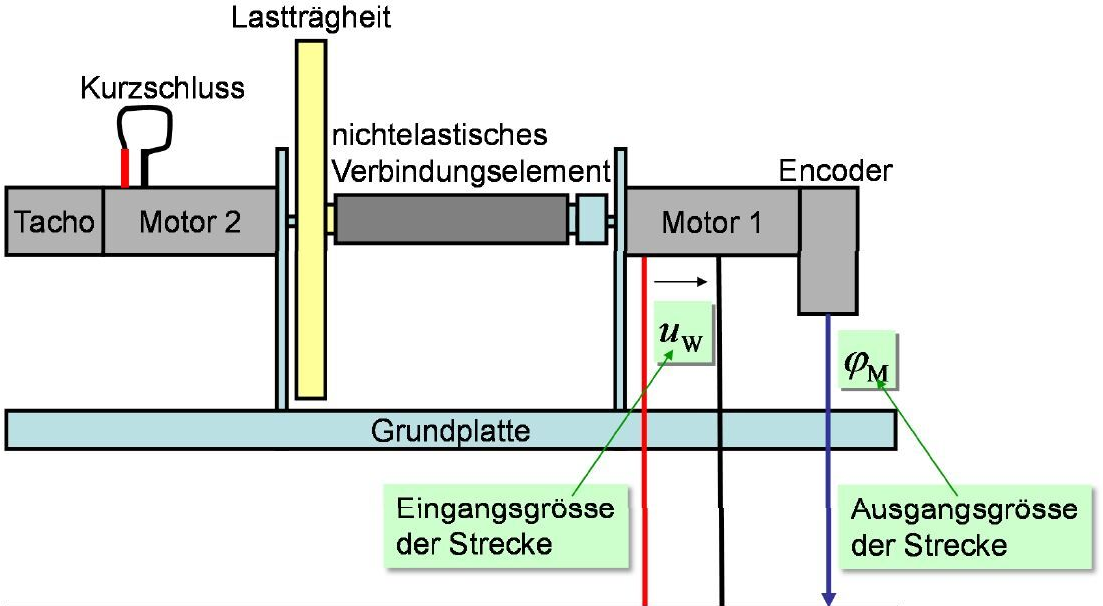
\includegraphics[width=14.5cm]{images/motor_baugruppe.png} %TODO anpassen
\caption{Motor-Baugruppe}
\label{Ab:motor-baugruppe}
\end{figure}

\section{Aufbau/Überblick}
Was brauchen wir?
\begin{itemize}
\item beschreibung von Simulationsmodell
\item beschreibung für Darstellung von Modell
\end{itemize}
erwähnen man braucht auch beschreibung wenn arbeiten ohne sim

Parameter für Model aus Datenblättern für die einzelnen Komponenten entnommen. %TODO ref anhang
Berechnung dämpfung
Für Parameter die nicht im Datenblatt stehen oder nicht genügend Informationen für eine Berechnung vorhanden ist, wurden geschätzt.
Jedoch haben diese  
%Somit haben wir folgende Werte die für die physikalische Beschreibung des Modells.
Für jeden Link müssen immer die Masse und der Trägheits-tensor definiter sein. Dabei darf die Masse nicht 0 sein und %TODO abklären inertia = 0 

\section{Gazebo}
\subsection{Gazebo Plugins}
beschreiben für was die Plugins sind, wie sie eingesetzt werden


\section{rviz}
\subsection{Joint State Publisher}
erklären für was gebraucht wird

\section{rqt}
keine speziellen anpassungen an urdf 



